\documentclass[11pt,a4paper]{ctexart}
\usepackage{geometry}
\geometry{margin=2cm}
\usepackage{amsmath,amssymb}
\usepackage{graphicx}
\usepackage{booktabs}
\usepackage{xcolor}
\usepackage[most]{tcolorbox}
\usepackage{hyperref}

\hypersetup{
    colorlinks=true,
    linkcolor=blue,
    filecolor=magenta,      
    urlcolor=cyan,
    pdftitle={流体力学：斜击波与斜激波习题汇总及完整解答},
}

% 定义优美的标题和排版样式
\title{\Huge \textbf{流体力学：斜击波（斜激波）习题汇总与完整解答}}
\author{\large 编写人：Antigravity \quad 适用课程：流体力学 / 空气动力学}
\date{\today}

% 自定义题目框
\newtcolorbox{questionbox}[2][]{
  colback=blue!3!white,
  colframe=blue!60!black,
  fonttitle=\bfseries,
  title={#2},
  boxrule=1pt,
  arc=3pt,
  halign title=flush left,
  #1
}

\begin{document}

\maketitle

\begin{abstract}
本篇文档精心挑选并整理了流体力学教学中关于\textbf{斜击波（斜激波）}与\textbf{普朗特-迈耶膨胀波}的5道典型计算题。题目均源自往年课程教学的经典例题及风洞、航空发动机设计中的真实问题。每道题目均附有详尽的推导公式、计算步骤以及相关的课件插图，旨在帮助学习者深入理解超声速流动中强扰动波的形成机理、波前后参数的变化规律及在工程实际中的设计应用。
\end{abstract}

\tableofcontents
\newpage

\section{斜击波（斜激波）基本计算关系式}
在进行习题求解前，首先给出定常、无粘、完全气体（以空气为例，比热比 $\gamma = 1.4$）通过斜击波的基本关系式，供计算查阅。
设斜击波前马赫数为 $Ma_1$，击波角为 $\beta$，气流经过击波后的偏转角为 $\delta$，则：
\begin{enumerate}
    \item \textbf{法向马赫数关系}：
    击波前法向马赫数：
    \begin{equation}
        Ma_{1n} = Ma_1 \sin \beta
    \end{equation}
    击波后法向马赫数：
    \begin{equation}
        Ma_{2n} = Ma_2 \sin (\beta - \delta)
    \end{equation}
    法向马赫数满足一维正激波关系式：
    \begin{equation}
        Ma_{2n}^2 = \frac{2 + (\gamma - 1)Ma_{1n}^2}{2\gamma Ma_{1n}^2 - (\gamma - 1)} = \frac{2 + 0.4 Ma_{1n}^2}{2.8 Ma_{1n}^2 - 0.4}
    \end{equation}
    
    \item \textbf{激波前后热力学参数比}（仅由法向分量决定）：
    压强比：
    \begin{equation}
        \frac{p_2}{p_1} = 1 + \frac{2\gamma}{\gamma+1}(Ma_{1n}^2 - 1) = \frac{2\gamma Ma_{1n}^2 - (\gamma - 1)}{\gamma+1}
    \end{equation}
    密度与速度法向分量比：
    \begin{equation}
        \frac{\rho_2}{\rho_1} = \frac{V_{1n}}{V_{2n}} = \frac{(\gamma+1)Ma_{1n}^2}{2 + (\gamma-1)Ma_{1n}^2}
    \end{equation}
    温度比：
    \begin{equation}
        \frac{T_2}{T_1} = \frac{p_2}{p_1} \frac{\rho_1}{\rho_2}
    \end{equation}
    
    \item \textbf{$\beta-\delta-Ma_1$ 关系式}（确定几何偏转与激波角）：
    \begin{equation}
        \tan \delta = 2 \cot \beta \frac{Ma_1^2 \sin^2 \beta - 1}{Ma_1^2 (\gamma + \cos 2\beta) + 2}
    \end{equation}
\end{enumerate}

\newpage

\section{习题集与完整解答}

% --- QUESTION 1 ---
\begin{questionbox}{题一：单尖楔对称绕流斜击波计算（单楔形绕流）}
超声速空气流（空气 $\gamma=1.4$，比热 $c_p = 1005\text{ J/(kg}\cdot\text{K)}$）以马赫数 $Ma_1 = 2.0$、静压 $p_1 = 69\text{ kPa}$ 绕流半顶角为 $\theta = 10^\circ$ 的对称尖楔。在其前缘尖端处产生附体弱斜击波。求：
\begin{enumerate}
    \item 弱斜击波的激波角 $\beta$；
    \item 击波后的马赫数 $Ma_2$；
    \item 击波后的静压 $p_2$。
\end{enumerate}
\end{questionbox}

\subsubsection*{【分析与解答】}
\begin{enumerate}
    \item \textbf{确定激波角 $\beta$}：
    已知来流马赫数 $Ma_1 = 2.0$，气流转角 $\delta = \theta = 10^\circ$。
    查 $\beta-\delta-Ma$ 关系曲线（或公式求解，见图\ref{fig:wedge_single}）：
    由 $Ma_1 = 2.0$ 和 $\delta = 10^\circ$，可求得两个激波角解，分别对应弱激波解和强激波解：
    \begin{align*}
        \beta_{\text{weak}} &\approx 39.3^\circ \quad (\text{实际流场中通常出现的弱解}) \\
        \beta_{\text{strong}} &\approx 84.0^\circ \quad (\text{对应波后为亚声速的强解，通常仅在下游有强烈阻塞时出现})
    \end{align*}
    本题取弱斜击波解：$\beta \approx 39.3^\circ$。

    \item \textbf{计算波后马赫数 $Ma_2$}：
    首先计算波前法向马赫数 $Ma_{1n}$：
    \[
    Ma_{1n} = Ma_1 \sin \beta = 2.0 \times \sin 39.3^\circ \approx 2.0 \times 0.6334 = 1.267
    \]
    将 $Ma_{1n} = 1.267$ 代入正激波关系式，求得波后法向马赫数 $Ma_{2n}$：
    \[
    Ma_{2n} = \sqrt{\frac{2 + 0.4 Ma_{1n}^2}{2.8 Ma_{1n}^2 - 0.4}} = \sqrt{\frac{2 + 0.4 \times 1.267^2}{2.8 \times 1.267^2 - 0.4}} = \sqrt{\frac{2.642}{4.093}} \approx 0.8032
    \]
    因此，波后真实马赫数 $Ma_2$ 为：
    \[
    Ma_2 = \frac{Ma_{2n}}{\sin(\beta - \delta)} = \frac{0.8032}{\sin(39.3^\circ - 10^\circ)} = \frac{0.8032}{\sin 29.3^\circ} \approx \frac{0.8032}{0.4894} \approx 1.640
    \]
    
    \item \textbf{计算波后静压 $p_2$}：
    利用法向马赫数求击波前后的压力比：
    \[
    \frac{p_2}{p_1} = 1 + \frac{2\gamma}{\gamma + 1}(Ma_{1n}^2 - 1) = 1 + \frac{2.8}{2.4}(1.267^2 - 1) \approx 1 + 1.1667 \times (1.605 - 1) \approx 1.707
    \]
    所以击波后的静压为：
    \[
    p_2 = 1.707 \times p_1 = 1.707 \times 69\text{ kPa} \approx 117.78\text{ kPa}
    \]
\end{enumerate}

\begin{figure}[htbp]
    \centering
    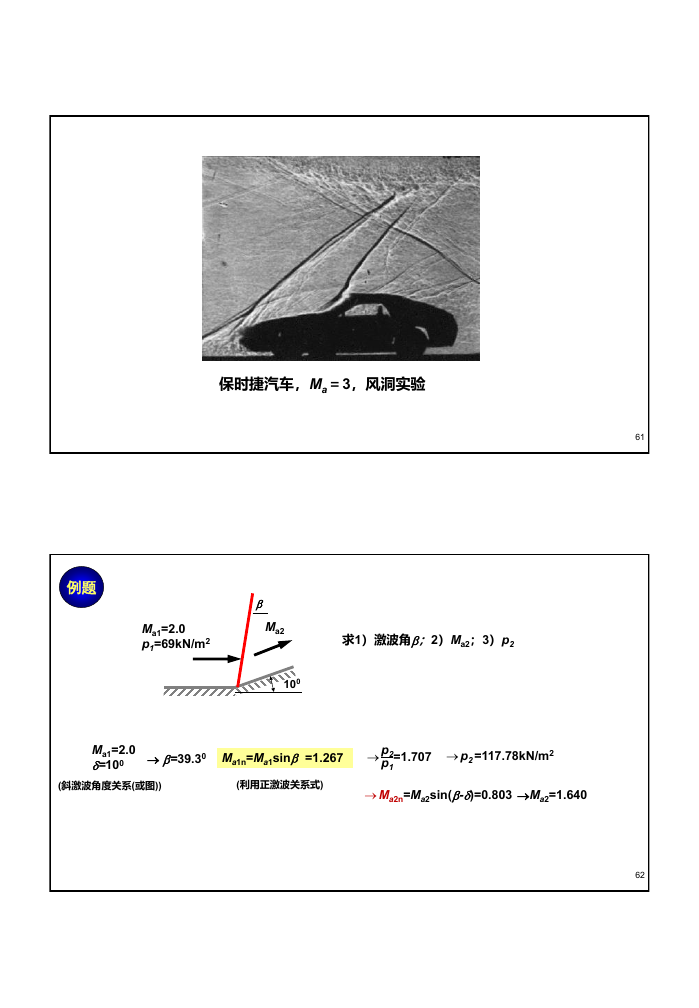
\includegraphics[width=0.65\textwidth]{oblique_shock_assets/wedge_single.png}
    \caption{单楔形折角超声速绕流与斜激波参数计算课件截图}
    \label{fig:wedge_single}
\end{figure}

\newpage

% --- QUESTION 2 ---
\begin{questionbox}{题二：双折角壁面相继压缩流动（双斜击波计算）}
超声速空气流（$\gamma=1.4$），波年来流马赫数为 $Ma_1 = 3.0$。流动相继流经两个转折角均为 $\theta_2 = \theta_3 = 10^\circ$ 的壁面折角，分别产生两级斜击波。若已知第一级斜击波的激波角为 $\beta_1 = 28.0^\circ$，第二级斜击波的激波角为 $\beta_2 = 33.0^\circ$。求：
\begin{enumerate}
    \item 第一级斜击波后的流动马赫数 $Ma_2$；
    \item 第二级斜击波后的流动马赫数 $Ma_3$。
\end{enumerate}
\end{questionbox}

\subsubsection*{【分析与解答】}
对于连续折角壁面，气流相继发生两次压缩。求解时必须以前一级的波后参数作为后一级的波前参数。

\begin{enumerate}
    \item \textbf{第一级斜击波后的流动马赫数 $Ma_2$}：
    已知波前马赫数 $Ma_1 = 3.0$，激波角 $\beta_1 = 28.0^\circ$，气流转角 $\theta_2 = 10^\circ$。
    - 第一级波前法向马赫数：
      \[
      Ma_{1n} = Ma_1 \sin \beta_1 = 3.0 \times \sin 28^\circ \approx 3.0 \times 0.4695 = 1.408
      \]
    - 波后法向马赫数 $Ma_{2n}$：
      \[
      Ma_{2n} = \sqrt{\frac{2 + 0.4 Ma_{1n}^2}{2.8 Ma_{1n}^2 - 0.4}} = \sqrt{\frac{2 + 0.4 \times 1.408^2}{2.8 \times 1.408^2 - 0.4}} = \sqrt{\frac{2.793}{5.149}} \approx 0.7365
      \]
    - 波后真实马赫数 $Ma_2$：
      \[
      Ma_2 = \frac{Ma_{2n}}{\sin(\beta_1 - \theta_2)} = \frac{0.7365}{\sin(28^\circ - 10^\circ)} = \frac{0.7365}{\sin 18^\circ} \approx \frac{0.7365}{0.3090} \approx 2.38
      \]

    \item \textbf{第二级斜击波后的流动马赫数 $Ma_3$}：
    经过第一级压缩后，流动转为平行于第一个斜面。此时波前马赫数为 $Ma_2 = 2.38$。气流再次偏转 $\theta_3 = 10^\circ$，激波角为 $\beta_2 = 33.0^\circ$。
    - 第二级波前法向马赫数：
      \[
      Ma_{2n}' = Ma_2 \sin \beta_2 = 2.38 \times \sin 33^\circ \approx 2.38 \times 0.5446 \approx 1.296
      \]
    - 第二级波后法向马赫数 $Ma_{3n}$：
      \[
      Ma_{3n} = \sqrt{\frac{2 + 0.4 Ma_{2n}'^2}{2.8 Ma_{2n}'^2 - 0.4}} = \sqrt{\frac{2 + 0.4 \times 1.296^2}{2.8 \times 1.296^2 - 0.4}} = \sqrt{\frac{2.672}{4.300}} \approx 0.788
      \]
    - 最终波后真实马赫数 $Ma_3$：
      \[
      Ma_3 = \frac{Ma_{3n}}{\sin(\beta_2 - \theta_3)} = \frac{0.788}{\sin(33^\circ - 10^\circ)} = \frac{0.788}{\sin 23^\circ} \approx \frac{0.788}{0.3907} \approx 2.01
      \]
\end{enumerate}

\begin{figure}[htbp]
    \centering
    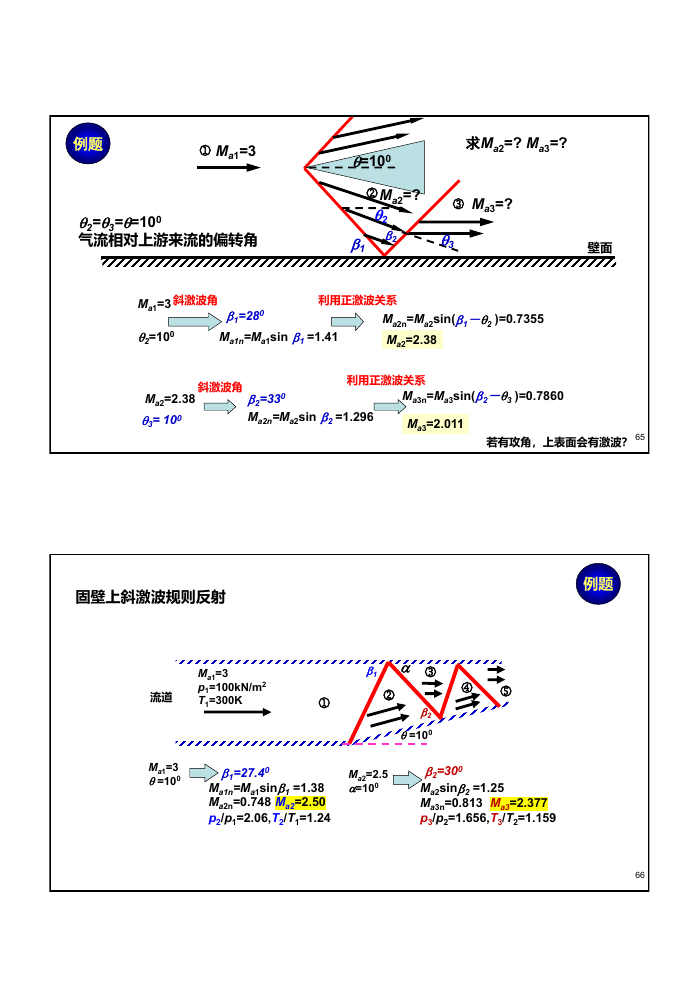
\includegraphics[width=0.65\textwidth]{oblique_shock_assets/wedge_double.png}
    \caption{多折角/双斜击波及规则反射流动分析课件截图}
    \label{fig:wedge_double}
\end{figure}

\newpage

% --- QUESTION 3 ---
\begin{questionbox}{题三：斜击波在平行固壁上的规则反射}
一均匀超声速空气来流马赫数 $Ma_1 = 3.0$，静压 $p_1 = 100\text{ kPa}$，温度 $T_1 = 300\text{ K}$。气流流过一个折角为 $\theta = 10^\circ$ 的壁面后产生一道斜击波。该击波入射到相对的平行平板固壁上并发生规则反射（如图\ref{fig:wedge_double}所示）。已知入射激波角为 $\beta_1 = 27.4^\circ$，反射激波角为 $\beta_2 = 30.0^\circ$。求：
\begin{enumerate}
    \item 入射波后（区域2）的参数 $Ma_2$、$p_2$ 和 $T_2$；
    \item 反射波后（区域3）的参数 $Ma_3$、$p_3$ 和 $T_3$。
\end{enumerate}
\end{questionbox}

\subsubsection*{【分析与解答】}
斜击波在固体表面反射时，为满足壁面无穿透边界条件，流动在通过反射击波后必须发生反向转折，转折角大小等于入射激波引起的气流偏转角，即 $\alpha = \theta = 10^\circ$。

\begin{enumerate}
    \item \textbf{求解入射波后（区域2）参数}：
    入射波前 $Ma_1 = 3.0$，$p_1 = 100\text{ kPa}$，$T_1 = 300\text{ K}$，$\beta_1 = 27.4^\circ$，$\theta = 10^\circ$。
    - 法向马赫数 $Ma_{1n}$：
      \[
      Ma_{1n} = Ma_1 \sin \beta_1 = 3.0 \times \sin 27.4^\circ \approx 3.0 \times 0.4602 = 1.38
      \]
    - 波后法向马赫数 $Ma_{2n}$：
      \[
      Ma_{2n} = \sqrt{\frac{2 + 0.4 \times 1.38^2}{2.8 \times 1.38^2 - 0.4}} \approx 0.748
      \]
    - 区域2的真实马赫数 $Ma_2$：
      \[
      Ma_2 = \frac{Ma_{2n}}{\sin(\beta_1 - \theta)} = \frac{0.748}{\sin(27.4^\circ - 10^\circ)} = \frac{0.748}{\sin 17.4^\circ} \approx \frac{0.748}{0.299} \approx 2.50
      \]
    - 静压 $p_2$：
      \[
      \frac{p_2}{p_1} = 1 + \frac{2.8}{2.4}(Ma_{1n}^2 - 1) = 1 + 1.1667 \times (1.38^2 - 1) \approx 2.06
      \]
      \[
      p_2 = 2.06 \times p_1 = 2.06 \times 100\text{ kPa} = 206\text{ kPa}
      \]
    - 温度 $T_2$：
      利用完全气体激波前后温度比关系：
      \[
      \frac{T_2}{T_1} = \frac{p_2}{p_1} \frac{\rho_1}{\rho_2} = \frac{p_2}{p_1} \times \frac{2 + (\gamma - 1)Ma_{1n}^2}{(\gamma + 1)Ma_{1n}^2} = 2.06 \times \frac{2 + 0.4 \times 1.38^2}{2.4 \times 1.38^2} \approx 2.06 \times 0.6033 \approx 1.24
      \]
      \[
      T_2 = 1.24 \times T_1 = 1.24 \times 300\text{ K} = 372\text{ K}
      \]

    \item \textbf{求解反射波后（区域3）参数}：
    反射波的波前来流即为区域2的流动参数：$Ma_2 = 2.50$，$p_2 = 206\text{ kPa}$，$T_2 = 372\text{ K}$。为使区域3的流动恢复平行于反射壁面，偏转角必须为 $\alpha = 10^\circ$（向相反方向折回）。已知反射波激波角 $\beta_2 = 30.0^\circ$。
    - 反射波前法向马赫数 $Ma_{2n}'$：
      \[
      Ma_{2n}' = Ma_2 \sin \beta_2 = 2.50 \times \sin 30.0^\circ = 1.25
      \]
    - 反射波后法向马赫数 $Ma_{3n}$：
      \[
      Ma_{3n} = \sqrt{\frac{2 + 0.4 \times 1.25^2}{2.8 \times 1.25^2 - 0.4}} = \sqrt{\frac{2.625}{3.975}} \approx 0.813
      \]
    - 区域3的真实马赫数 $Ma_3$：
      \[
      Ma_3 = \frac{Ma_{3n}}{\sin(\beta_2 - \alpha)} = \frac{0.813}{\sin(30.0^\circ - 10.0^\circ)} = \frac{0.813}{\sin 20.0^\circ} \approx \frac{0.813}{0.3420} \approx 2.38
      \]
    - 区域3的静压 $p_3$：
      \[
      \frac{p_3}{p_2} = 1 + \frac{2.8}{2.4}(Ma_{2n}'^2 - 1) = 1 + 1.1667 \times (1.25^2 - 1) \approx 1.656
      \]
      \[
      p_3 = 1.656 \times p_2 = 1.656 \times 206\text{ kPa} \approx 341.14\text{ kPa}
      \]
    - 区域3的温度 $T_3$：
      \[
      \frac{T_3}{T_2} = \frac{p_3}{p_2} \times \frac{2 + (\gamma - 1)Ma_{2n}'^2}{(\gamma + 1)Ma_{2n}'^2} = 1.656 \times \frac{2 + 0.4 \times 1.25^2}{2.4 \times 1.25^2} = 1.656 \times \frac{2.625}{3.75} \approx 1.1592
      \]
      \[
      T_3 = 1.1592 \times T_2 = 1.1592 \times 372\text{ K} \approx 431.2\text{ K}
      \]
\end{enumerate}

\newpage

% --- QUESTION 4 ---
\begin{questionbox}{题四：超声速进气道多波系减速方案设计与对比（总压恢复比）}
为了将马赫数 $Ma_1 = 3.0$ 的超声速空气流减速为亚声速流动（以供喷气发动机燃烧室使用），设计师考虑了两种进气道方案（如图\ref{fig:inlet_comparison}所示）：
\begin{description}
    \item[方案一]：流体直接通过一道正击波减速为亚声速。
    \item[方案二]：流体首先通过一个激波角为 $\beta = 40.0^\circ$ 的斜击波（对应气流偏转角 $\delta = 22.0^\circ$）进行预压缩，然后再通过一道正击波减速为亚声速。
\end{description}
求两种方案的最终总压恢复比 $p_{0,\text{exit}}/p_{01}$，并从流动损失的角度讨论方案二的设计优势及其工程实际意义。
\end{questionbox}

\subsubsection*{【分析与解答】}
总压恢复比 $p_{0,\text{exit}}/p_{01}$ 是衡量超声速进气道效率的最重要指标。总压损失越小，说明流动过程的效率越高，能量可用性保持得越好。

\begin{enumerate}
    \item \textbf{方案一：直接正击波减速}：
    对于 $Ma_1 = 3.0$ 的一维正击波，直接查正击波表（或用公式计算公式）可得其滞止压力比（总压恢复比）：
    \[
    \left(\frac{p_{02}}{p_{01}}\right)_{\text{case 1}} \approx 0.3283
    \]
    这说明直接通过正击波减速，气流将损失掉高达 $67.17\%$ 的总压。

    \item \textbf{方案二：斜击波 + 正击波减速}：
    \begin{itemize}
        \item \textbf{第一阶段：斜击波压缩}：
        来流 $Ma_1 = 3.0$，击波角 $\beta = 40.0^\circ$。
        法向马赫数 $Ma_{1n} = Ma_1 \sin \beta = 3.0 \times \sin 40.0^\circ \approx 3.0 \times 0.6428 = 1.928$。
        以 $Ma_{1n} = 1.928$ 查正击波表，得到斜击波前后的总压比：
        \[
        \frac{p_{02}}{p_{01}} \approx 0.7535
        \]
        斜击波后的法向马赫数 $Ma_{2n} \approx 0.588$。
        斜击波后的真实马赫数 $Ma_2$ 为：
        \[
        Ma_2 = \frac{Ma_{2n}}{\sin(\beta - \delta)} = \frac{0.588}{\sin(40.0^\circ - 22.0^\circ)} = \frac{0.588}{\sin 18^\circ} \approx \frac{0.588}{0.3090} \approx 1.90
        \]
        
        \item \textbf{第二阶段：正击波压缩}：
        气流以 $Ma_2 = 1.90$ 通过第二道正击波。
        查 $Ma = 1.90$ 的正击波关系表，可得正击波前后的总压比为：
        \[
        \frac{p_{03}}{p_{02}} \approx 0.7674
        \]
        
        \item \textbf{最终总压比}：
        \[
        \left(\frac{p_{03}}{p_{01}}\right)_{\text{case 2}} = \frac{p_{02}}{p_{01}} \times \frac{p_{03}}{p_{02}} \approx 0.7535 \times 0.7674 \approx 0.5782
        \]
    \end{itemize}

    \item \textbf{讨论与结论}：
    对比两个方案的计算结果：
    \[
    \frac{\left(p_{03}/p_{01}\right)_{\text{case 2}}}{\left(p_{02}/p_{01}\right)_{\text{case 1}}} = \frac{0.5782}{0.3283} \approx 1.76
    \]
    方案二的总压恢复比是方案一的约 $1.76$ 倍！
    
    \textbf{工程实际意义}：
    激波的总压损失随激波强度的增强呈非线性剧烈增长。直接通过大马赫数（如 $Ma_1=3.0$）的正击波会造成灾难性的总压损失。
    方案二利用斜板产生斜击波，先将超声速气流适度减速（从 $Ma_1=3.0$ 降到 $Ma_2=1.9$），再让流速较低的超声速气流通过正击波。由于两道较弱激波的总压损失之和远小于单道强激波的损失，进气道整体效率得以显著提高。这正是现代超声速战斗机和高超声速飞行器进气道采用调节板产生“多级斜激波预压缩+弱正激波终压缩”设计方案的物理本源。
\end{enumerate}

\begin{figure}[htbp]
    \centering
    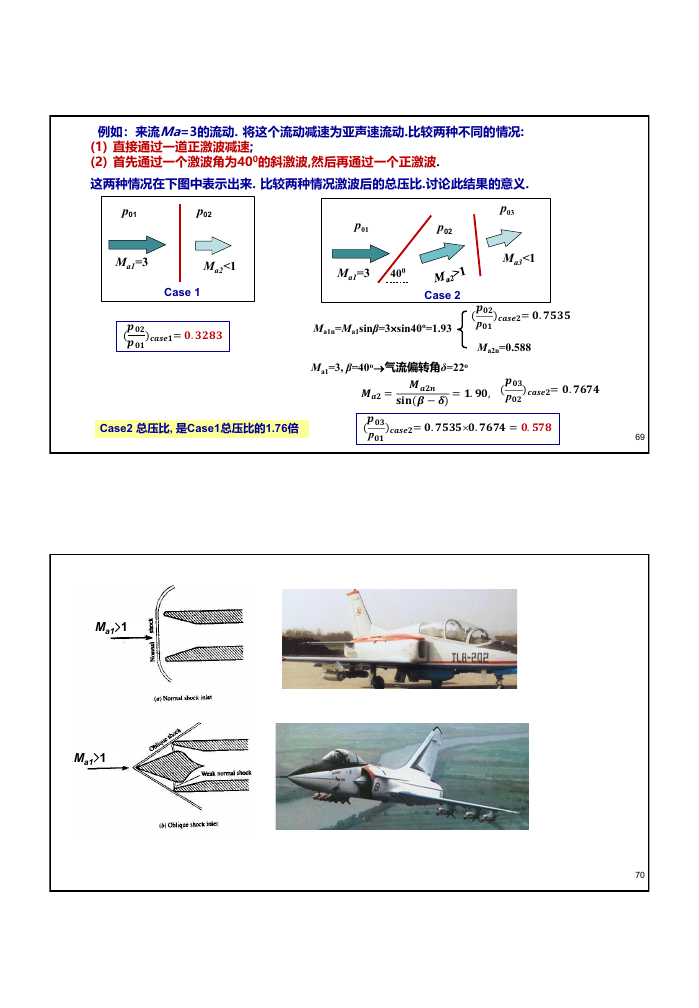
\includegraphics[width=0.7\textwidth]{oblique_shock_assets/inlet_comparison.png}
    \caption{进气道中直接正击波减速（Case 1）与斜+正双击波减速（Case 2）方案对比课件截图}
    \label{fig:inlet_comparison}
\end{figure}

\newpage

% --- QUESTION 5 ---
\begin{questionbox}{题五：高超声速风洞流场诊断与斜击波物理机理}
在高超声速风洞（来流介质为空气，$\gamma = 1.4$）中进行某尖锐模型超声速绕流实验，通过纹影法拍摄到如图\ref{fig:wind_tunnel}所示的流场。观测到模型前缘产生了一道附体斜击波。
已知测得激波倾角（斜击波角） $\beta = 19.0^\circ$，激波后的气流偏转角 $\delta = 13.0^\circ$，来流马赫数 $Ma_1 = 7.53$，波后流动马赫数 $Ma_2 = 4.95$。请分析解答：
\begin{enumerate}
    \item 计算激波前的法向马赫数 $Ma_{1n}$ 以及激波后的法向马赫数 $Ma_{2n}$；
    \item 阐明在斜击波分析中，为什么可以将速度进行分解并套用一维正激波公式或正激波表来计算波前后的热力学参数比值（如压强比 $p_2/p_1$, 密度比 $\rho_2/\rho_1$ 等）；
    \item 为什么正激波表中的总压比公式 $p_{02}/p_1 = f(Ma_1)$ 在斜击波中绝对不可直接套用来计算 $p_{02}/p_1$？
\end{enumerate}
\end{questionbox}

\subsubsection*{【分析与解答】}
\begin{enumerate}
    \item \textbf{法向马赫数的计算}：
    - 击波前沿法向马赫数：
      \[
      Ma_{1n} = Ma_1 \sin \beta = 7.53 \times \sin 19.0^\circ \approx 7.53 \times 0.3256 \approx 2.452
      \]
    - 击波后沿法向马赫数：
      \[
      Ma_{2n} = Ma_2 \sin(\beta - \delta) = 4.95 \times \sin(19.0^\circ - 13.0^\circ) = 4.95 \times \sin 6.0^\circ \approx 4.95 \times 0.1045 \approx 0.517
      \]
    注意，由于 $Ma_{1n} = 2.452 > 1.0$，法向流动是超声速的，满足激波产生的条件。波后的法向流动减速为亚声速（$Ma_{2n} = 0.517 < 1.0$），但由于保留了很大的切向速度分量，真实马赫数 $Ma_2 = 4.95$ 依然处于高超声速状态。

    \item \textbf{斜击波物理分解的理论依据}：
    建立紧贴斜击波的控制体，将气流速度 $V$ 分解为垂直于击波面的法向速度 $V_n$ 和平行于击波面的切向速度 $V_t$。
    - \textbf{切向动量守恒}：由于激波是一个面，击波面法向存在强烈的压强梯度，但切向没有压力差。在无粘流体假设下，切向受力为零，因而切向动量守恒，即：
      \[
      V_{1t} = V_{2t}
      \]
    - \textbf{法向守恒方程}：切向速度的守恒使其在动量方程和能量方程中可以被消去。法向的质量守恒、动量守恒和能量守恒方程在形式上与一维正激波完全一致（仅需将绝对流速 $V$ 替换为法向速度 $V_n$）。
    因此，任何单纯由法向压缩决定的热力学参数比值（如压强比 $p_2/p_1$、密度比 $\rho_2/\rho_1$、温度比 $T_2/T_1$ 以及法向马赫数的关系）都仅与法向分量有关。我们可以通过令 $Ma_{1n} = Ma_1 \sin\beta$ 代替正激波公式中的波前马赫数，直接查正激波表或应用正激波公式进行求解。

    \item \textbf{总压比 $p_{02}/p_1$ 不可直接套用的原因}：
    总压 $p_0$ 的定义是流体等熵滞止（速度减为零）时的压强：
    \[
    p_0 = p \left(1 + \frac{\gamma - 1}{2} Ma^2\right)^{\frac{\gamma}{\gamma-1}}
    \]
    一维正激波表中给出的 $p_{02}/p_1$ 是指\textbf{全部速度 $V_2$ 被滞止时的总压} $p_{02}$ 与波前静压 $p_1$ 的比值。
    而在斜击波中，如果我们把 $Ma_{1n}$ 误作为波前马赫数去查正激波表中的 $p_{02}/p_1$，其物理意义代表的是\textbf{仅仅将法向速度分量 $V_{2n}$ 滞止到零，而切向速度分量 $V_{2t}$ 仍保持不变时的压强}（通常称为法向总压 $p_{02n}$）与 $p_1$ 的比值。由于忽略了切向速度的动能贡献，这样求得的 $p_{02n}$ 远小于流体全部滞止时的真实总压 $p_{02}$。
    
    因此，计算斜击波的总压恢复比 $p_{02}/p_{01}$ 可以用法向马赫数 $Ma_{1n}$ 查正激波表（因为总温 $T_{01} = T_{02}$，且切向滞止是可逆等熵的，故法向总压之比与真实总压之比相等：$p_{02}/p_{01} = p_{02n}/p_{01n}$）；但绝不能用 $Ma_{1n}$ 去直接查正激波表里的 $p_{02}/p_1$。
\end{enumerate}

\begin{figure}[htbp]
    \centering
    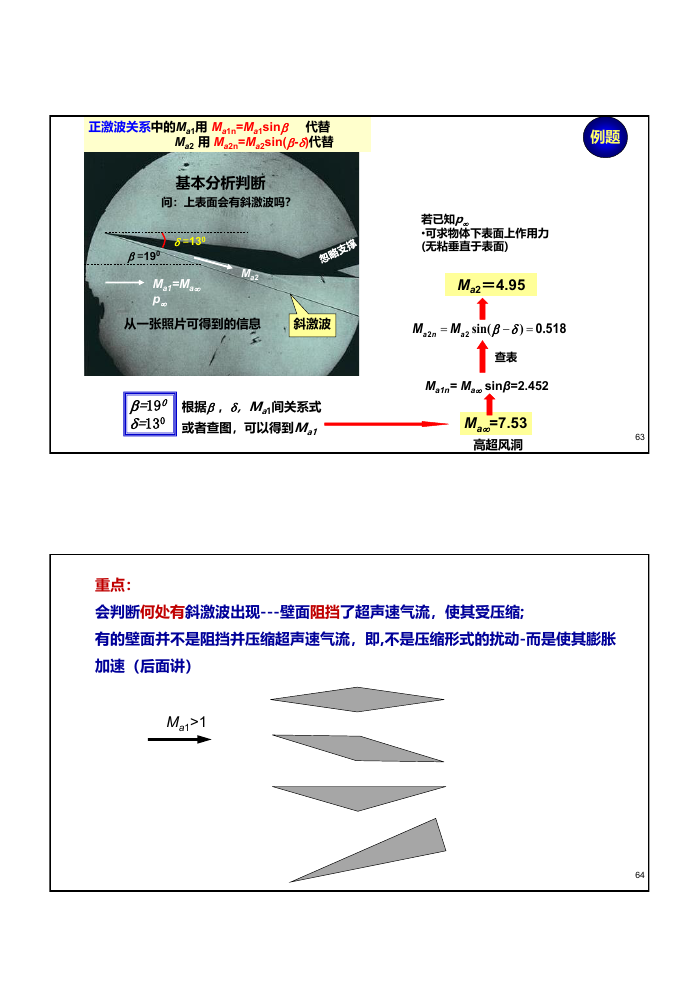
\includegraphics[width=0.7\textwidth]{oblique_shock_assets/wind_tunnel.png}
    \caption{高超声速风洞实验中的斜击波现象截图}
    \label{fig:wind_tunnel}
\end{figure}

\end{document}
